\documentclass[11pt]{article}

\usepackage[margin=1in]{geometry}
\usepackage{amsmath,amssymb,amsthm}
\usepackage{booktabs}
\usepackage{enumitem}
\usepackage{graphicx}
\usepackage{hyperref}
\usepackage{microtype}
\usepackage{parskip}
\usepackage{placeins}
\usepackage{float}
\usepackage[font=small,labelfont=bf]{caption}
\usepackage{tikz}
\usepackage{pgfplots}
\pgfplotsset{compat=1.18}
\usetikzlibrary{arrows.meta}

\hypersetup{colorlinks=true, linkcolor=blue, citecolor=blue, urlcolor=blue}
\setlength{\emergencystretch}{3em}
\allowdisplaybreaks

\definecolor{figblue}{HTML}{2A6FB0}
\definecolor{figorange}{HTML}{D1622B}
\definecolor{figteal}{HTML}{1D9E75}
\definecolor{figpurple}{HTML}{534AB7}
\definecolor{figink}{HTML}{242424}
\definecolor{figboxgray}{HTML}{A0A0A0}
\definecolor{figlightgray}{HTML}{E8E8E8}
\definecolor{figpaleteal}{HTML}{E8F4F0}
\definecolor{figpalepurple}{HTML}{F1EEFB}

\pgfplotsset{
  every axis/.append style={
    line width=0.5pt,
    axis line style={black!70},
    tick style={line width=0.4pt, black!60},
    label style={font=\small},
    tick label style={font=\footnotesize},
    legend style={font=\footnotesize, draw=none, fill=none},
  },
}

\newtheorem{theorem}{Theorem}[section]
\newtheorem{proposition}[theorem]{Proposition}
\newtheorem{lemma}[theorem]{Lemma}
\newtheorem{corollary}[theorem]{Corollary}
\newtheorem{definition}[theorem]{Definition}

\newcommand{\val}{\operatorname{val}}
\newcommand{\gap}{\operatorname{gap}}
\newcommand{\tol}{\tau_0}

\title{An Exact Approach to Solving the Drop the Handkerchief Game}
\author{James Cenawood\thanks{Code and instructions to reproduce the results
are available in the project repository.}}
\date{August 25, 2026}

\begin{document}
\maketitle

\begin{abstract}
Drop the Handkerchief (DTH) is a death game in the final arc ``Surpassing
The Leader'' of the manga \textit{Usogui} by Toshio Sako. It is a two-player,
zero-sum stochastic game with simultaneous actions and full observation. We
solve the complete 60-action timing model under the frozen survival law of
Section~\ref{sec:game}. After a player can no longer survive an injection,
the game does not read their cumulative time dead (TTD) again. A quotient by
that fact collapses the $5.27\times10^{9}$ states to $289{,}374{,}121$
classes. A potential function puts the classes into $1{,}201$ layers, and one
backward sweep solves them.

Each value has a mixed-strategy gap of at most $10^{-6}$ against its full
$60\times60$ stage matrix. The matrix is triangular Toeplitz, so one 59-step
recurrence gives both equilibrium strategies. One source file builds the
whole table in $49$ seconds on a fifteen-core laptop. At the root state
$V=0.08985\pm0.00061$, so the first Dropper wins with probability
$0.54493\pm0.00031$ under optimal play.
\end{abstract}

\section{Introduction}
DTH is the pure timing core of the Surpassing the Leader arc wager in
\emph{Usogui}. Two players alternate as \emph{Dropper} and \emph{Checker}.
In each round, both players choose a second in $\{1,\dots,60\}$. A successful
check adds the inclusive delay to the Checker's squandered time (ST), and
then the roles swap. A failed check injects that ST plus sixty seconds. The
Checker revives with the probability in Figure~\ref{fig:revival}, or loses.

The game is finite but large, and each round can need a mixed strategy. The
solution has four steps:

\begin{enumerate}[leftmargin=*]
\item quotient the profiles for which failure is certainly fatal
  (Section~\ref{sec:quotient});
\item rank every transition with a potential that always increases
  (Section~\ref{sec:potential});
\item solve each $60\times60$ stage game from its $61$ different entries and
  keep a gap certificate (Sections~\ref{sec:stage} and~\ref{sec:certified});
\item run the sweep as one fused kernel over each layer
  (Section~\ref{sec:computation}).
\end{enumerate}

At a state $x$, each player chooses a distribution over the sixty seconds:
\[
\Delta_{60}=\left\{\sigma\in\mathbb R^{60}:\sigma_i\ge0,
\ \sum_{i=1}^{60}\sigma_i=1\right\}.
\]
The stage matrix $M(x)$ gives the payoff of each action pair, so
\[
V(x)=\max_{\sigma_d\in\Delta_{60}}\min_{\sigma_c\in\Delta_{60}}
\sigma_d^{\mathsf T}M(x)\sigma_c.
\]
Each entry of the matrix is a terminal payoff or the value of a later state.
When the transitions form a DAG, the later values substitute backward. Since
$V=P(\mathrm{win})-P(\mathrm{loss})$, $P(\mathrm{win})=(1+V)/2$.

\section{The game}\label{sec:game}

\begin{definition}[State]\label{def:state}
A player's \emph{profile} is $z=(s,t)$: the current ST and TTD. A live state
is the ordered pair $x=(z_c,z_d)=(s_c,t_c,s_d,t_d)$ from the view of the
current \emph{Dropper}, with $s_c,s_d\in\{0,\dots,299\}$ and
$t_c,t_d\in\{0,\dots,300\}$. The terminal payoff is $+1$ if the current
Dropper wins and $-1$ if they lose. Values are from the view of the current
Dropper and negate when the roles swap.
\end{definition}

\begin{definition}[Actions and timing]\label{def:actions}
Both players choose seconds $d,c\in\{1,\dots,60\}$ at the same time (drop
and check). The check \emph{succeeds} if and only if $d\le c$. Then the
Checker's ST grows by the inclusive interval $\ell=c-d+1\in\{1,\dots,60\}$;
equal seconds cost one second, not zero. If $s_c+\ell\ge300$, the cylinder
overflows and the Dropper gets payoff $+1$. If not, play continues with the
roles swapped:
\[
(s_c,t_c,s_d,t_d)\ \xrightarrow{\ \text{success, lag }\ell\ }\
(s_d,\,t_d,\,s_c+\ell,\,t_c).
\]
\end{definition}

\begin{definition}[Failure, dose, and revival]\label{def:failure}
On a failed check ($d>c$) the Checker gets the dose $q=s_c+60$. Survival is
possible if and only if
\begin{equation}\label{eq:survive}
q<300\ \wedge\ q+t_c\le300
\qquad\Longleftrightarrow\qquad
s_c\le239\ \wedge\ s_c+t_c\le240 .
\end{equation}
A profile is \emph{revival-eligible} when \eqref{eq:survive} holds and
\emph{failure-fatal} when it does not. Both terms describe the next failed
check; both players are alive in a live state. A revival-eligible Checker
revives with probability
\begin{equation}\label{eq:revival}
p(s_c,t_c)\;=\;0.95\left(1-\frac{s_c}{240}\right)0.75^{\,t_c/60}.
\end{equation}
Then the cylinder resets and the TTD absorbs the dose:
\[
(s_c,t_c,s_d,t_d)\ \xrightarrow{\ \text{failure, revive}\ }\
(s_d,\,t_d,\,0,\,t_c+s_c+60)
\quad\text{with probability }p(s_c,t_c).
\]
If not, the transition ends with payoff $+1$. When \eqref{eq:survive} fails,
$p\equiv0$.
\end{definition}

The source fixes the shape of \eqref{eq:revival}: the vial plus sixty
seconds against a five-minute cap, and revival prospects that decrease with
accumulated deaths~\cite{stlevidence}. It does not fix linearity, the product
form, or the constants $0.95$ and $0.75$; those are choices of the model. A
coarse six-action sensitivity check moved the baseline $0.95$ alone across
$0.85$--$0.99$. The root value moved by $0.0028$, and the Dropper's
first-action mass moved from $0.387$ to $0.257$. The value is stable to that
parameter; the policy is not.

\begin{figure}[t]
\centering
\includegraphics[width=0.8\textwidth]{build/figures/seaborn/fig1_revival_probability.pdf}
\caption{The frozen revival law \eqref{eq:revival}. Color and height both
show probability. The blue edge is the linear loss from ST. The purple edge is
the exponential loss from TTD. The pale plateau is the zero-probability
region, which contains $(240,240)$. The orange curtain marks $s+t=240$:
probability is positive on the curtain, except at $s=240$, and is zero beyond
it.}
\label{fig:revival}
\end{figure}

\section{Finiteness and stage structure}\label{sec:stage}

\begin{lemma}[Damage increases]\label{lem:damage}
Let $R(x)=s_c+t_c+s_d+t_d$. Every live transition increases $R$. A
successful lag $\ell$ adds $\ell\ge1$. A revived failure adds exactly $60$.
\end{lemma}

\begin{corollary}[The game is finite]\label{cor:finite}
$R\le1198$ on live states, so every play ends within $1199$ transitions.
Thus every live state has a unique value $V(x)\in[-1,1]$. Backward induction
over the finite acyclic transition graph gives it~\cite{zermelo1913}, with
von Neumann's minimax theorem at each state~\cite{vonneumann1928}. The
construction is the finite, absorbing case of a Shapley stochastic
game~\cite{shapley1953}.
\end{corollary}

\begin{proposition}[The 61 transition classes]\label{prop:classes}
Fix a live state $x$ and let $V$ give the values of its children. Write the
Dropper's continuation payoff after a success of lag $\ell$, or after a
failure, as
\begin{align*}
S_\ell&=
\begin{cases}
+1,& s_c+\ell\ge300,\\
-V(s_d,t_d,s_c+\ell,t_c),&\text{else},
\end{cases}\\[3pt]
F&=
\begin{cases}
+1,& (s_c,t_c)\ \text{failure-fatal},\\
p\,\bigl(-V(s_d,t_d,0,t_c+s_c+60)\bigr)+(1-p),&\text{else}.
\end{cases}
\end{align*}
Then the stage matrix of $x$, with the Dropper as the row player, is
\begin{equation}\label{eq:toeplitz}
M(x)_{d,c}=
\begin{cases}
S_{c-d+1}, & c\ge d,\\
F, & c<d,
\end{cases}
\end{equation}
and $V(x)=\val(M(x))$. $M(x)$ has at most $61$ different entries: it is
Toeplitz on and above the diagonal and constant below it.
\end{proposition}

\begin{proof}
A successful cell depends on the actions only through the lag $\ell=c-d+1$.
Every failed cell has the same transition distribution. The entries are the
expected continuation values, negated for the role swap.
\end{proof}

\begin{lemma}[Constant-time saddle test]\label{lem:toeplitz}
Row $d$ of \eqref{eq:toeplitz} contains the prefix $S_1,\dots,S_{61-d}$, and
also $F$ when $d>1$. Column $c$ contains the prefix $S_1,\dots,S_c$, and also
$F$ when $c<60$. Let $m=\min_\ell S_\ell$ and $\overline m=\max_\ell S_\ell$.
Then
\[
\max_d\min_c M(x)_{d,c}=\max\bigl(m,\ \min(S_1,F)\bigr),
\qquad
\min_c\max_d M(x)_{d,c}=\min\bigl(\overline m,\ \max(S_1,F)\bigr).
\]
Among rows $d>1$, the row minimum is largest at $d=60$. Among columns
$c<60$, the column maximum is smallest at $c=1$. The test is exact, because
min and max select one of their arguments and add no rounding.
\end{lemma}

Figure~\ref{fig:toeplitz} shows the layout. Each row contains a prefix of the
$S$ array, never an arbitrary subset. Thus the minimum and the maximum of the
$60$ success values, plus two comparisons, give every row minimum and column
maximum. The matrix is never built.

\begin{figure}[t]
\centering
\includegraphics[width=0.92\textwidth]{build/figures/seaborn/fig2_toeplitz_structure.pdf}
\caption{An $8\times8$ view of the stage matrix \eqref{eq:toeplitz}. The lag
$\ell=c-d+1$ is constant on each diagonal. Every failed check has the value
$F$. Row minima and column maxima reduce to prefix scans of $S$
(Lemma~\ref{lem:toeplitz}), with the same result as a scan of all $3{,}600$
cells.}
\label{fig:toeplitz}
\end{figure}

\section{The failure-fatal quotient}\label{sec:quotient}

The model reads a player's TTD only in the revival probability
\eqref{eq:revival}. After failure becomes fatal, the exact TTD has no more
effect. Profiles $(250,60)$ and $(250,300)$ both get dose $310$ on a failed
check, and success only raises ST. Thus they can share the sentinel
$(250,\bot)$.

\begin{lemma}[Failure-fatality is absorbing]\label{lem:absorbing}
If $(s,t)$ is failure-fatal, then $(s',t)$ is failure-fatal for every
$s'\ge s$. A successful check raises ST and keeps TTD. A failed check ends
the game for that player, or needs \eqref{eq:survive}. Thus no transition
makes the profile revival-eligible again.
\end{lemma}

\begin{theorem}[Quotient soundness]\label{thm:quotient}
Let $\varphi(s,t)=(s,t)$ when $(s,t)$ is revival-eligible and
$\varphi(s,t)=(s,\bot)$ when it is not, applied to each player's profile
independently. Two live states with equal images under $\varphi$ have
identical stage matrices up to $\varphi$-identification of their children.
Thus they have identical values: $V$ factors through $\varphi$.
\end{theorem}

\begin{proof}
Compare the $61$ classes of Proposition~\ref{prop:classes} at two states that
differ only in a failure-fatal player's TTD. Success classes do not read TTD.
A child's $\varphi$-image depends only on the parent's image and $\ell$
(Lemma~\ref{lem:absorbing}). The failure class reads the Checker's TTD only
through $p$. A failure-fatal Checker gives $F=+1$ with no child, and a
revival-eligible Checker is not quotiented. Induction over the finite acyclic
graph completes the proof.
\end{proof}

\begin{proposition}[Counts and closure]\label{prop:count}
The root TTDs lie in $\{0\}\cup[60,300]$, and the domain is closed under
transitions. Revival needs $s_c+t_c\le240$, so a failure child's TTD
$t_c+s_c+60$ lies in $[60,300]$; success keeps TTDs. Over this domain,
one player has $300\times242=72{,}600$ profiles. The quotient keeps all
$16{,}711$ revival-eligible profiles and replaces the failure-fatal TTDs at
each ST with one sentinel. This leaves $17{,}011$ classes per player and
\[
17{,}011^2=289{,}374{,}121
\]
two-player classes, against $72{,}600^2=5{,}270{,}760{,}000$ before the
quotient. A revival-eligible profile with TTD in $1..59$ is unreachable, and
the implementation rejects it.
\end{proposition}

Figure~\ref{fig:quotient} shows why the reduction is large. Revival-eligible
profiles are $23\%$ of the one-player domain. Both profiles are
revival-eligible in only $5.3\%$ of states.

\begin{figure}[H]
\centering
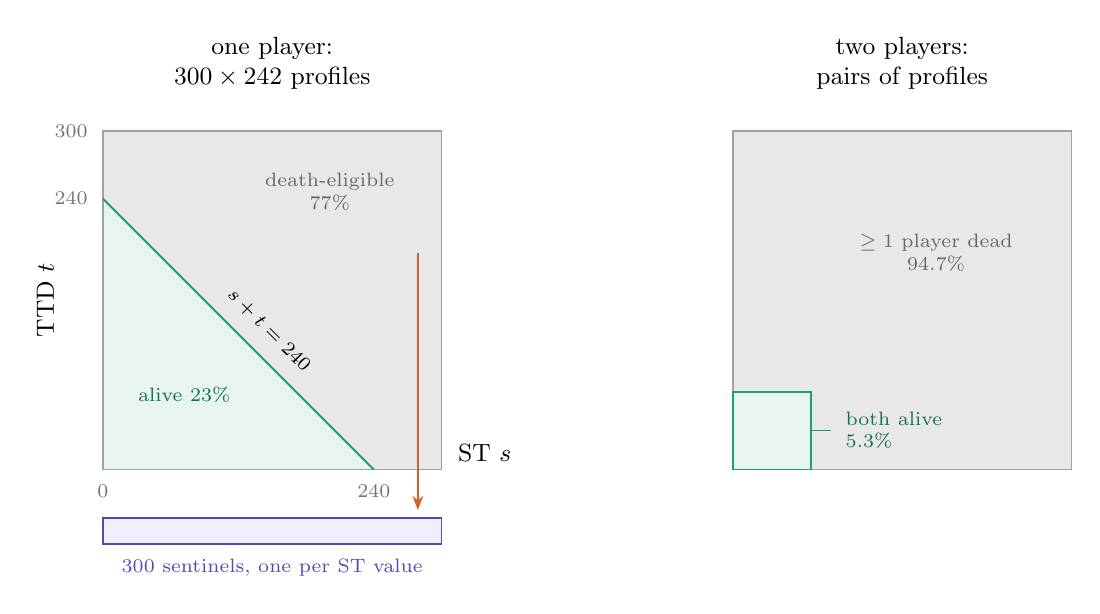
\begin{tikzpicture}[x=0.86cm, y=0.86cm]
\fill[figlightgray] (0,0) rectangle (5,5);
\fill[figpaleteal] (0,0) -- (4,0) -- (0,4) -- cycle;
\draw[figboxgray, line width=0.5pt] (0,0) rectangle (5,5);
\draw[figteal, line width=0.7pt] (4,0) -- (0,4);
\node[font=\scriptsize, rotate=-45] at (2.45,2.05) {$s+t=240$};
\node[font=\scriptsize, text=figteal!70!black] at (1.2,1.1)
  {alive $23\%$};
\node[font=\scriptsize, align=center, text=figink!70] at (3.35,4.1)
  {death-eligible\\$77\%$};
\fill[figpalepurple] (0,-1.1) rectangle (5,-0.72);
\draw[figpurple, line width=0.6pt]
  (0,-1.1) rectangle (5,-0.72);
\draw[-{Stealth[length=1.8mm]}, figorange, line width=0.8pt]
  (4.65,3.2) -- (4.65,-0.6);
\node[font=\scriptsize, text=figpurple, anchor=north] at (2.5,-1.18)
  {$300$ sentinels, one per ST value};
\node[font=\scriptsize, text=black!55, anchor=north] at (0,-0.08) {$0$};
\node[font=\scriptsize, text=black!55, anchor=north] at (4,-0.08) {$240$};
\node[font=\scriptsize, text=black!55, anchor=east] at (-0.08,4) {$240$};
\node[font=\scriptsize, text=black!55, anchor=east] at (-0.08,5) {$300$};
\node[font=\small, anchor=west] at (5.1,0.25) {ST $s$};
\node[font=\small, rotate=90] at (-0.85,2.5) {TTD $t$};
\node[font=\small, align=center] at (2.5,6.0)
  {one player:\\ $300\times242$ profiles};
\begin{scope}[xshift=8cm]
\fill[figlightgray] (0,0) rectangle (5,5);
\fill[figpaleteal] (0,0) rectangle (1.15,1.15);
\draw[figboxgray, line width=0.5pt] (0,0) rectangle (5,5);
\draw[figteal, line width=0.7pt] (0,0) rectangle (1.15,1.15);
\node[font=\scriptsize, align=center, text=figink!70] at (3.0,3.2)
  {$\geq 1$ player dead\\$94.7\%$};
\draw[figteal, line width=0.6pt] (1.15,0.575) -- (1.45,0.575);
\node[font=\scriptsize, align=left, text=figteal!70!black, anchor=west]
  at (1.52,0.575) {both alive\\$5.3\%$};
\node[font=\small, align=center] at (2.5,6.0)
  {two players:\\ pairs of profiles};
\end{scope}
\end{tikzpicture}
\caption{The quotient for one player (left) and for pairs of players
(right). Each vertical fibre in the death-eligible region collapses to one
sentinel per ST value. The left panel is schematic, because TTD values
$1,\dots,59$ are unreachable. The percentages are exact counts on the closed
domain. ``Death-eligible'' and ``dead'' mean failure-fatal. Neither means that
a player has left the game.}
\label{fig:quotient}
\end{figure}

\section{The potential and the sweep schedule}\label{sec:potential}

The potential is not payoff, value, or strategic advantage. It is only a
progress score that orders the states.

\begin{definition}[Potential]\label{def:potential}
For a profile let $\rho(s,t)=t$ if $(s,t)$ is revival-eligible and
$\rho(s,t)=301$ if it is not. For a class let
\[
\Phi(x)=s_c+s_d+\rho(s_c,t_c)+\rho(s_d,t_d)\in\{0,\dots,1200\}.
\]
\end{definition}

\begin{theorem}[Strict increase]\label{thm:potential}
Every live transition increases $\Phi$. The cases for the profile that moves
are:
\begin{itemize}[leftmargin=*]
\item successful lag $\ell$, same side of the revival boundary:
  $\Delta\Phi=\ell\ge1$;
\item successful lag $\ell$, the profile becomes failure-fatal:
  $\Delta\Phi=\ell+301-t\ge\ell+61$, because revival-eligibility implies
  $t\le240$;
\item failure, the revived profile stays revival-eligible: $\Delta\Phi=60$,
  because ST resets while TTD absorbs the dose;
\item failure, the revived profile becomes failure-fatal:
  $\Delta\Phi=301-(s_c+t_c)\ge61$ by \eqref{eq:survive}.
\end{itemize}
\end{theorem}

\begin{corollary}[Layered backward induction]\label{cor:layers}
No transition stays inside a $\Phi$-layer. Thus a descending sweep solves
every child before its parents. With the one-player bucket
$B_a=\{(s,t):s+\rho(s,t)=a\}$, layer $P$ is exactly
\[
\Phi^{-1}(P)=
\bigcup_{\substack{0\le a\le600\\0\le P-a\le600}}B_a\times B_{P-a}.
\]
The $289{,}374{,}121$ classes fill all $1{,}201$ layers. The largest layer,
$\Phi=374$, holds $1{,}678{,}715$ classes.
\end{corollary}

The classes form the layered DAG in Figure~\ref{fig:potential-dag}. The table
build asserts the increase over every profile transition. The schedule needs
no reachability analysis, frontier queue, or transposition table, and it
solves unreachable classes too.

\begin{figure}[H]
\centering
\begin{tikzpicture}[
  x=1cm,
  y=1cm,
  state/.style={circle, draw=figblue, fill=white, line width=0.7pt,
    minimum size=6mm, inner sep=0pt},
  focus/.style={state, draw=figteal, fill=figpaleteal, line width=0.9pt},
  edge/.style={-{Stealth[length=1.7mm]}, draw=figblue!75!black,
    line width=0.65pt},
  rank/.style={draw=figlightgray, dashed, line width=0.55pt},
]
\begin{scope}[yshift=2.85cm, yscale=0.72]
\draw[rank] (1.2,0.55) -- (1.2,3.75);
\draw[rank] (4.5,0.55) -- (4.5,3.75);
\draw[rank] (7.8,0.55) -- (7.8,3.75);
\draw[rank] (11.1,0.55) -- (11.1,3.75);
\node[font=\small] at (1.2,4.35) {$\Phi=P$};
\node[font=\small] at (4.5,4.35) {$\Phi=P+a$};
\node[font=\small] at (7.8,4.35) {$\Phi=P+b$};
\node[font=\small] at (11.1,4.35) {$\Phi=P+c$};
\node[state] (a1) at (1.2,1.00) {};
\node[focus] (a2) at (1.2,2.20) {$x$};
\node[state] (a3) at (1.2,3.40) {};
\node[state] (b1) at (4.5,0.80) {};
\node[state] (b2) at (4.5,1.70) {};
\node[state] (b3) at (4.5,2.70) {};
\node[state] (b4) at (4.5,3.60) {};
\node[state] (c1) at (7.8,1.00) {};
\node[state] (c2) at (7.8,2.20) {};
\node[state] (c3) at (7.8,3.40) {};
\node[state] (d1) at (11.1,1.35) {};
\node[state] (d2) at (11.1,3.05) {};
\draw[edge] (a1) -- (b1);
\draw[edge] (a1) -- (b2);
\draw[edge] (a2) -- (b2);
\draw[edge] (a2) -- (b3);
\draw[edge] (a2) -- (c2);
\draw[edge] (a3) -- (b3);
\draw[edge] (a3) -- (b4);
\draw[edge] (b1) -- (c1);
\draw[edge] (b2) -- (c1);
\draw[edge] (b2) -- (c2);
\draw[edge] (b3) -- (c2);
\draw[edge] (b3) -- (c3);
\draw[edge] (b4) -- (c3);
\draw[edge] (c1) -- (d1);
\draw[edge] (c2) -- (d1);
\draw[edge] (c2) -- (d2);
\draw[edge] (c3) -- (d2);
\draw[-{Stealth[length=2mm]}, draw=figpurple, line width=0.95pt]
  (11.1,0.10) -- (1.2,0.10);
\node[font=\scriptsize, text=figpurple, fill=white, inner sep=2pt]
  at (6.15,0.10) {backward solve};
\end{scope}
\begin{axis}[
  at={(0cm,0cm)}, anchor=south west,
  width=12.25cm, height=2.15cm,
  scale only axis,
  xmin=0, xmax=1200, ymin=0, ymax=1900000,
  axis lines=left,
  xlabel={potential layer $\Phi$},
  ylabel={classes},
  xtick={0,300,600,900,1200},
  ytick={0,800000,1600000},
  yticklabels={0,$0.8$M,$1.6$M},
  scaled y ticks=false,
  label style={font=\scriptsize},
  tick label style={font=\scriptsize},
  grid=major,
  grid style={draw=figlightgray, line width=0.4pt},
  clip=false,
]
\addplot[draw=figblue, fill=figblue!14, line width=0.75pt]
  table[x=potential, y=classes] {build/figures/layer_widths.dat}
  \closedcycle;
\addplot[only marks, mark=*, mark size=1.7pt, figorange]
  coordinates {(374,1678715)};
\node[anchor=south west, font=\scriptsize, text=figorange]
  at (axis cs:374,1678715) {peak: $1.68$M};
\end{axis}
\end{tikzpicture}
\caption{Top: some transitions in the potential-ranked DAG. Bottom: the exact
width of all $1{,}201$ layers on a linear scale. Every edge points right; the
computation runs from right to left.}
\label{fig:potential-dag}
\end{figure}

\section{Certified equilibria}\label{sec:certified}

\begin{definition}[Certificate]\label{def:certificate}
For a stage matrix $M$ and mixed strategies $\sigma_d$ (Dropper) and
$\sigma_c$ (Checker), let
\[
L=\min_c(\sigma_d^{\mathsf T}M)_c,\qquad
U=\max_d(M\sigma_c)_d,\qquad
\gap_M(\sigma_d,\sigma_c)=\max(0,\,U-L).
\]
The pair \emph{certifies} the value $\widehat v=(L+U)/2$ at tolerance $\tol$
when $\gap_M(\sigma_d,\sigma_c)\le\tol$. In this paper $\tol=10^{-6}$. The
gap is always measured against the full matrix \eqref{eq:toeplitz}.
\end{definition}

\begin{proposition}[Certified midpoint]\label{prop:midpoint}
$L\le\val(M)\le U$ for every mixed pair. Thus a certificate at tolerance
$\tol$ gives $|\widehat v-\val(M)|\le\tol/2$. If
$\max_{d,c}|M_{d,c}-\widehat M_{d,c}|\le\epsilon$, then
$|\val(M)-\val(\widehat M)|\le\epsilon$.
\end{proposition}

\begin{proposition}[One recurrence, both strategies]\label{prop:equalizer}
Let $d_0=S_1-F$ and $\Delta_m=S_{m+1}-S_m$. If $d_0\ne0$, define
\[
r_1=1,\qquad
r_k=-\frac{1}{d_0}\sum_{m=1}^{k-1}\Delta_m\,r_{k-m}\quad(k=2,\dots,60).
\]
Then $\sigma_d\propto(r_1,\dots,r_{60})$ makes $\sigma_d^{\mathsf T}M$
constant, $\sigma_c\propto(r_{60},\dots,r_1)$ makes $M\sigma_c$ constant,
and $(M\sigma_c)_i=(\sigma_d^{\mathsf T}M)_{61-i}$ for every $i$.
\end{proposition}

\begin{proof}
Row $d+1$ of \eqref{eq:toeplitz} is row $d$ moved one column to the right,
with $F$ in column $d$. Thus, for $d=1,\dots,59$,
\[
(M\sigma_c)_d-(M\sigma_c)_{d+1}
=d_0\,\sigma_{c,d}+\sum_{m\ge1}\Delta_m\,\sigma_{c,d+m}.
\]
This is zero when the Dropper is indifferent between seconds $d$ and $d+1$.
Zero gives $\sigma_{c,d}$ from the later entries. Start at
$\sigma_{c,60}=1$ and step down $59$ times: this is the recurrence with
$r_k=\sigma_{c,61-k}$. The same subtraction on columns $c$ and $c+1$ gives
$d_0\,\sigma_{d,c+1}+\sum_{m\ge1}\Delta_m\,\sigma_{d,c+1-m}$, the same
coefficients read forwards from $\sigma_{d,1}=1$, so $\sigma_{d,k}=r_k$.
Substitute $k\mapsto61-k$ in the two sums to get
$(M\sigma_c)_i=(\sigma_d^{\mathsf T}M)_{61-i}$.
\end{proof}

Negative entries of $r$ are clipped, and the pair is normalized, before the
certificate is measured. The clip cannot invalidate the bounds, because they
hold for any mixed pair. Each class then goes through the same ladder:

\begin{enumerate}[leftmargin=*]
\item \textbf{Pure saddle.} Lemma~\ref{lem:toeplitz}. If the maximin and the
  minimax meet within $\tol$, a pure action pair is enough.
\item \textbf{Equalizer.} Proposition~\ref{prop:equalizer}: $1{,}770$
  multiply-adds for $r$ and $1{,}770$ for $M\sigma_c$. Its maximum and
  minimum are $U$ and $L$.
\item \textbf{Linear programming.} The standard zero-sum program
  $\max\{v:M^{\mathsf T}\sigma_d\ge v\mathbf1,\ \mathbf1^{\mathsf T}\sigma_d=1,
  \ \sigma_d\ge0\}$, with $\sigma_c$ from its duals, then the same
  full-matrix check.
\end{enumerate}

\begin{proposition}[A priori accumulated bound]\label{prop:accumulated}
Let every stored value have a certificate at tolerance $\tol$. Let
$\delta(x)$ bound the longest live path from $x$ to a terminal. Then
\[
|\widehat V(x)-V(x)|\;\le\;\delta(x)\,\frac{\tol}{2}
\;\le\;\frac{1201-\Phi(x)}{2}\,\tol ,
\]
so the root state obeys $|\widehat V-V|(0,0,0,0)\le6.1\times10^{-4}$.
\end{proposition}

\begin{proof}
Induction up the DAG. Terminal entries are exact. If every child is within
$(\delta(x)-1)\tol/2$ of truth, then the assembled matrix is within that
distance entrywise, because expectation and negation are non-expansive.
Proposition~\ref{prop:midpoint} moves the bound to the value and adds the
state's own $\tol/2$. Theorem~\ref{thm:potential} bounds $\delta$.
\end{proof}

\begin{proposition}[Full-policy bound]\label{prop:policy}
Let $\widehat\pi$ play the accepted pair at every class. Let
$\underline V_{\widehat\pi}(x)$ and $\overline V_{\widehat\pi}(x)$ be its
security values against every complete opposing policy, with deviations
after later role swaps included. Then
\[
\overline V_{\widehat\pi}(x)-\underline V_{\widehat\pi}(x)
\le\varepsilon(x)\le(1201-\Phi(x))\tol,
\]
where $\varepsilon(x)=(U_x-L_x)+\max_y\varepsilon(y)$ over live children
$y$, and $\varepsilon=0$ at terminals. At the root state, no unilateral
deviation improves the win probability by more than $6.005\times10^{-4}$.
\end{proposition}

\begin{proof}
At a terminal, both security values equal $\widehat V$. Assume the two
bounds for every live child $y$:
$\underline V_{\widehat\pi}(y)\ge\widehat V(y)-\tfrac12\varepsilon(y)$ and
$\overline V_{\widehat\pi}(y)\le\widehat V(y)+\tfrac12\varepsilon(y)$.
Negation at the role swap and the average after revival keep the largest
child bound. Thus
$\underline V_{\widehat\pi}(x)\ge L_x-\tfrac12\max_y\varepsilon(y)$ and
$\overline V_{\widehat\pi}(x)\le U_x+\tfrac12\max_y\varepsilon(y)$. With
$\widehat V(x)=(L_x+U_x)/2$, this is the recurrence for $\varepsilon$.
\end{proof}

\begin{figure}[t]
\centering
\begin{tikzpicture}
\begin{axis}[
  width=0.95\textwidth, height=3.9cm,
  xlabel={second}, ylabel={probability},
  xmin=0, xmax=61, ymin=0.005, ymax=0.35,
  ymode=log,
  log ticks with fixed point,
  ytick={0.005,0.01,0.03,0.1,0.3},
  yticklabel style={/pgf/number format/fixed},
  legend style={at={(0.5,0.97)}, anchor=north, legend columns=2},
]
\addplot[figblue, line width=0.8pt, mark=*, mark size=1pt]
  table[x=action, y=drop] {build/figures/root_strategies.dat};
\addplot[figorange, dashed, line width=0.8pt, mark=*, mark size=1pt]
  table[x=action, y=check] {build/figures/root_strategies.dat};
\legend{Dropper $\sigma_d$, Checker $\sigma_c$}
\end{axis}
\end{tikzpicture}
\caption{The first-round strategies of the selected full-game policy, both
with full support. The Dropper puts $27.3\%$ on second $1$, and a ramp from
$0.6\%$ to $2.2\%$ on the other seconds. The Checker is the exact mirror
$\sigma_{c,j}=\sigma_{d,61-j}$ of Proposition~\ref{prop:equalizer}.
Proposition~\ref{prop:policy} shows how later gaps accumulate.}
\label{fig:root}
\end{figure}

\section{The computation}\label{sec:computation}

The implementation is one Python file of $476$ lines. It builds the
$17{,}011$ quotient profiles with their successful-check children, failure
child, and revival probability. It stores $V$ as a $17{,}011\times17{,}012$
float64 array. The extra column holds $-1$, so a terminal win reads as $+1$
after the role-swap negation, with no branch. It lists each layer by
Corollary~\ref{cor:layers}, in an order where consecutive classes read the
same row of $V$. One compiled kernel per layer runs in parallel over the
classes.

For each class, the kernel gathers the $61$ continuation values. It runs
Lemma~\ref{lem:toeplitz}, then Proposition~\ref{prop:equalizer}, in
sixty-entry scratch that stays in first-level cache. It tracks the minimum
and the maximum of $M\sigma_c$ as they are produced. It writes the certified
midpoint and its rung. Classes that fail both rungs are collected and solved
by linear programming afterwards.

\subsection{Results}

The sweep covered all $289{,}374{,}121$ classes in $48.9$ seconds on an
Apple M5 Pro laptop. The laptop has five performance cores and ten efficiency
cores; the kernel used fifteen threads with a static schedule. That is about
$5.9$ million classes per second, and a single thread does $0.49$ million
per second. The earlier artifact came from the same rules on a twelve-core
desktop: $5{,}432$ seconds for $98.1\%$ of the table. It used a warm-started
support search, two bordered $61\times61$ linear systems per class, and
sessions with checkpoints.

Three changes explain the ratio. Proposition~\ref{prop:equalizer} replaces
about $1.6\times10^{5}$ floating-point operations per class with about
$3.6\times10^{3}$. The fused kernel removes every temporary array. The clip
of the equalizer, in place of a rejection, sends no class to the linear
program.

\begin{center}
\begin{tabular}{@{}lrr@{}}
\toprule
rung & classes & share\\
\midrule
pure saddle (Lemma~\ref{lem:toeplitz}) & $334{,}177$ & $0.115\%$\\
equalizer (Proposition~\ref{prop:equalizer}) & $289{,}039{,}944$ & $99.885\%$\\
linear programming & $0$ & $0$\\
\bottomrule
\end{tabular}
\end{center}

\noindent
The earlier artifact sent $190{,}995$ classes to linear programming and
$334{,}588$ to the pure rung. The difference is borderline classes with a
gap at the tolerance; both routes are certified.

Six stored values were compared with the earlier artifact. Five agree to
within $2\times10^{-11}$; the state $(250,300,40,0)$ agrees to
$1.2\times10^{-9}$. After the sweep, an independent scalar ladder re-solved
$1{,}200$ evenly strided classes from their stored children. The largest
difference from the stored value was $8.9\times10^{-16}$. The root's local
gap is $5.6\times10^{-17}$. Figure~\ref{fig:root} shows its strategies.

\noindent\begin{minipage}{\textwidth}
\begin{theorem}[Main result]\label{thm:main}
The complete 60-action timing model of Section~\ref{sec:game} has a certified
numerical solution on the closed quotient domain of
Proposition~\ref{prop:count}. Every one of its $289{,}374{,}121$ classes has
a stored midpoint with local gap at most $10^{-6}$. At the root state the
stored midpoint is $0.0898500728141386$, and
\[
V(0,0,0,0)=0.08985\pm0.00061,
\qquad
P(\text{first Dropper wins})=0.54493\pm0.00031.
\]
For the selected full-game policy,
$\overline V_{\widehat\pi}(0,0,0,0)-\underline V_{\widehat\pi}(0,0,0,0)
\le1.201\times10^{-3}$.
\end{theorem}
\end{minipage}


\section{Scope of the claims}\label{sec:claims}

\begin{itemize}[leftmargin=*]
\item \textbf{Rules-relative.} The results concern Section~\ref{sec:game} and
  the frozen revival surface \eqref{eq:revival}. They do not concern the
  leap-aware game with its asymmetric 61st second.
\item \textbf{Certified numerics.} Values are round-to-nearest float64
  midpoints with saddle-gap certificates, not rational or interval
  arithmetic. The structural theorems are exact. The table build asserts
  survival, absorption, the counts, and the potential increase by
  enumeration.
\item \textbf{Domain.} States with a revival-eligible profile with TTD in
  $1..59$ are outside the table; the implementation rejects them.
\item \textbf{Policies.} The table stores values and routes;
  Proposition~\ref{prop:equalizer} re-derives strategies from child values in
  microseconds.
\end{itemize}

\textbf{Reproducibility.} From the repository root, \texttt{uv run
src/main.py} builds the table, re-solves the $1{,}200$ audit classes, and
prints the six reference values in about one minute. \texttt{uv run pytest}
runs the seventeen structural and numerical checks.

\vspace{-1.2em}
\begin{thebibliography}{9}
\footnotesize
\setlength{\itemsep}{0pt}

\bibitem{stlevidence}
Toshio Sako. \emph{Usogui}. Shueisha, 2006--2018.
\newblock Source evidence indexed in \emph{Canonical game evidence}, project
ledger entries E-CYLINDER-CAP, E-DOSE-COMPOSITION, E-PROXIMITY-RISK,
and E-TTD-SLACK, 2026.
\newblock \href{https://youngjump.jp/manga/usogui/}{Official series page.}

\bibitem{zermelo1913}
Ernst Zermelo.
\newblock \"Uber eine Anwendung der Mengenlehre auf die Theorie des
Schachspiels.
\newblock In \emph{Proceedings of the Fifth International Congress of
Mathematicians}, volume 2, pages 501--504, Cambridge, 1913.

\bibitem{vonneumann1928}
John von Neumann.
\newblock Zur Theorie der Gesellschaftsspiele.
\newblock \emph{Mathematische Annalen}, 100:295--320, 1928.
\newblock \href{https://doi.org/10.1007/BF01448847}{doi:10.1007/BF01448847}

\bibitem{shapley1953}
Lloyd S. Shapley.
\newblock Stochastic games.
\newblock \emph{Proceedings of the National Academy of Sciences},
39(10):1095--1100, 1953.
\newblock \href{https://doi.org/10.1073/pnas.39.10.1095}%
{doi:10.1073/pnas.39.10.1095}

\end{thebibliography}

\end{document}
